\chapter{Lennard Jones fluid}

\vspace{-1cm} \noindent \textcolor{graytitle}{\textit{{\Large The very basics of LAMMPS through a simple example}}\vspace{0.5cm} }

\noindent \hspace{-0.45cm}\begin{wrapfigure}{r}{4cm}
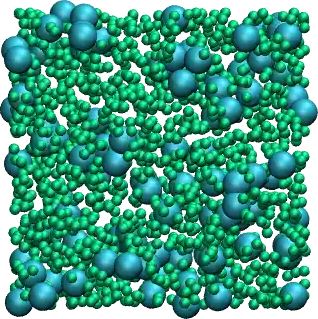
\includegraphics[width=4cm]{tutorials/level0/lennard-jones-fluid/binary_LJ_fluid_light.png}
\end{wrapfigure}

\noindent The objective of this tutorial is to use
LAMMPS to perform a simple molecular dynamics simulation
of a binary fluid in the NVT ensemble. The system is a simple Lennard-Jones fluid
made of neutral dots with a Langevin thermostating. The
simulation box is cubic with periodic boundary conditions.

This tutorial illustrates the use of several ingredients of
molecular dynamics simulations, such as system initialization,
energy minimization, integration of the equations of motion,
and trajectory visualization.

\section{The input script}

\noindent In order to run a simulation using LAMMPS, one needs to
write a series of commands in an input script. For clarity,
this script will be divided into five categories which we are going to
fill up one by one. 

Create a folder, call it \textit{my-first-input}, and then create a blank
text file in it, called \textit{input.lammps}.

Copy the following lines in \textit{my-first-input/input.lammps}, 
where a line starting with a brace ($\#$) is a comment
that is ignored by LAMMPS:

\begin{lcverbatim}
# PART A - ENERGY MINIMIZATION
# 1) Initialization
# 2) System definition
# 3) Simulation settings
# 4) Visualization
# 5) Run
\end{lcverbatim}

\noindent These five categories are not required in every
input script, and should not necessarily be in that
exact order. For instance parts 3 and 4 could be inverted, or
part 4 could be omitted. Note however that LAMMPS reads input
file from top to bottom, therefore the \textit{Initialization} and 
\textit{System definition} categories must appear at the top of the
input, and the \textit{Run} category at the bottom.

\subsection{System creation}

\noindent In the first section of the script, called \textit{Initialization},
let us indicate to LAMMPS the most basic information
about the simulation, such as:
\begin{itemize}
\item the conditions at the boundaries of the box (periodic, non-periodic, ...)
\item the type of atoms (uncharged single dots, spheres with angular velocities, ...).
\end{itemize}
Enter the following lines in \textit{my-first-input/input.lammps}:

\begin{lcverbatim}
# 1) Initialization
units lj
dimension 3
atom_style atomic
pair_style lj/cut 2.5
boundary p p p
\end{lcverbatim}

\noindent The first line, \textit{units lj}, indicates that we want to
use the system of unit called \textit{LJ}, for Lennard-Jones, for
which all quantities are unitless. 

\begin{tcolorbox}[colback=mylightblue!5!white,colframe=mylightblue!75!black,title=About Lennard-Jones (LJ) units]
Lennard-Jones (LJ) units are a dimensionless system of units.
LJ units are often used in molecular simulations
and theoretical calculations. When using LJ units:
\begin{itemize}
\item energies are expressed in units of $\epsilon$, where $\epsilon$ is the
  depth of the potential of the LJ interaction,
\item distances are expressed in units of $\sigma$, where $\sigma$ is the distance
  at which the particle-particle potential energy is zero,
\item masses are expressed in units of the atomic mass $m$.
\end{itemize}
All the other quantities are normalized by a combination of $\epsilon$, $\sigma$,
and $m$. For instance, time is expressed in units of $\sqrt{ \epsilon / m \sigma^2}$.
Find the full list of quantities \href{https://docs.lammps.org/units.html}{from the LAMMPS website}.

\end{tcolorbox}

\noindent The second line, \textit{dimension 3}, indicates that the simulation
is 3D. The third line, \textit{atom$\_$style atomic}, that the \textit{atomic} style
will be used, therefore each atom is just a dot with a mass.

\begin{tcolorbox}[colback=mylightblue!5!white,colframe=mylightblue!75!black,title=About the atom style]
While we are keeping it simple here,
in the following tutorials, different \textit{atom$\_$style} will be used,
allowing us to create atoms with a net charge and to define 
bonds between atoms to form molecules.
\end{tcolorbox}

\noindent The fourth line, \textit{pair$\_$style lj/cut 2.5}, indicates that atoms
are going to interact through a Lennard-Jones potential with
a cut-off equal to $r_c = 2.5$ (unitless):

$$E (r) = 4 \epsilon \left[ \left( \dfrac{\sigma}{r} \right)^{12} - \left( \dfrac{\sigma}{r} \right)^{6} \right], ~ \text{for} ~ r < r_c.$$

The last line, \textit{boundary p p p}, indicates that the
periodic boundary conditions will be used along all three
directions of space (the 3 \textit{p} stand for \textit{x}, \textit{y}, and \textit{z},
respectively).
At this point, \textit{my-first-input/input.lammps} is a 
LAMMPS input script that does nothing.
You can run it using LAMMPS to verify that the \textit{input} contains
no mistake by running the following command in the terminal
from the \textit{my-first-input/}  folder:

\begin{lcverbatim}
lmp -in input.lammps
\end{lcverbatim}

\noindent which should return:

\begin{lcverbatim}
LAMMPS (2 Aug 2023 - Update 1)
Total wall time: 0:00:00
\end{lcverbatim}

\noindent If there is a mistake in the input script, for example if
\textit{atom$\_$stile} is written instead of \textit{atom$\_$style}, LAMMPS
gives you an explicit warning:

\begin{lcverbatim}
LAMMPS (2 Aug 2023 - Update 1)
ERROR: Unknown command: atom_stile  atomic (src/input.cpp:232)
Last command: atom_stile atomic
\end{lcverbatim}

\noindent Let us fill the \textit{System definition} category of the input script:

\begin{lcverbatim}
# 2) System definition
region simulation_box block -20 20 -20 20 -20 20
create_box 2 simulation_box
create_atoms 1 random 1500 341341 simulation_box
create_atoms 2 random 100 127569 simulation_box
\end{lcverbatim}

\noindent The first line, \textit{region simulation$\_$box (...)}, creates a region
named \textit{simulation$\_$box} that is a block (i.e. a rectangular cuboid) that
extends from -20 to 20 (no unit) along all 3 directions of space.

The second line, , creates a simulation box based on
the region \textit{simulation$\_$box} with \textit{2} types of atoms.

The third line, \textit{create$\_$atoms (...)} creates 1500 atoms of type 1
randomly within the region \textit{simulation$\_$box}. The integer \textit{341341} is a
seed that can be changed in order to create different
initial conditions for the simulation. The fourth line
creates 100 atoms of type 2.
If you run LAMMPS, you should see the following information in the
terminal:

\begin{lcverbatim}
(...)
Created orthogonal box = (-20 -20 -20) to (20 20 20)
(...)
Created 1500 atoms
(...)
Created 100 atoms
(...)
\end{lcverbatim}

\noindent From what is printed in the terminal, it is clear that
LAMMPS correctly interpreted the commands, and first created
the box with desired dimensions, then 1500 atoms, then 100
atoms.
Let us fill the third section of the input script, the settings:

\begin{lcverbatim}
# 3) Simulation settings
mass 1 1
mass 2 1
pair_coeff 1 1 1.0 1.0
pair_coeff 2 2 0.5 3.0
\end{lcverbatim}

\noindent The two first commands attribute a mass
equal to 1 (unitless) to both atoms of type 1 and 2,
respectively. The third line sets the Lennard-Jones
coefficients for the interactions between atoms of type 1,
respectively the depth of the potential well
$\epsilon$ and the distance at which the
particle-particle potential energy is zero $\sigma$. 
The last line sets the Lennard-Jones coefficients for
the interactions between atoms of type 2.

\begin{tcolorbox}[colback=mylightblue!5!white,colframe=mylightblue!75!black,title=About cross parameters]
By default, LAMMPS calculates the cross coefficients between the different atom types
using geometric average: 
$\epsilon_{ij} = \sqrt{\epsilon_{ii} \epsilon_{jj}}$,
$\sigma_{ij} = \sqrt{\sigma_{ii} \sigma_{jj}}$. 
In the present case, and even without specifying it explicitly, we thus have:
\begin{itemize}
\item $\epsilon_{ij} = \sqrt{1.0 \times 0.5} = 0.707$, and 
\item $\sigma_{ij} = \sqrt{1.0 \times 3.0} = 1.732$.
\end{itemize}
Eventually, cross parameters could also be explicitly specified by adding the following 
line to the input file (but there is no need to do it here, its only necessary if you need 
to set custom parameters):
\begin{lcverbatim}

pair_coeff 1 2 0.707 1.732 
\end{lcverbatim}

\noindent Note that the arithmetic rule, where 
$\epsilon_{ij} = \sqrt{\epsilon_{ii} \epsilon_{jj}}$,
$\sigma_{ij} = (\sigma_{ii}+\sigma_{jj})/2$, 
is more common than the geometric rule. However, neither the geometric nor the
arithmetic rule are based on rigorous argument, so here
the geometric rule will do just fine. 
\end{tcolorbox}

\noindent \subsection{Energy minimization}

Now that the system is fully defined, let us just fill the two last remaining sections:

\begin{lcverbatim}
# 4) Visualization
thermo 10
# 5) Run
minimize 1.0e-4 1.0e-6 1000 10000
\end{lcverbatim}

\noindent The thermo command asks LAMMPS to print
thermodynamic information (e.g. temperature, energy) in the
terminal every 10 steps. The second line asks LAMMPS to
perform an energy minimization of the system.

\begin{tcolorbox}[colback=mylightblue!5!white,colframe=mylightblue!75!black,title=About energy minimization]
An energy minimization procedure consists in adjusting
the coordinates of the atoms that are too close from one another until one of the stopping
criteria is reached. By default, LAMMPS uses the conjugate gradient (CG) algorithm.
Here there are four stopping criteria:
\begin{itemize}
\item The change in energy between two iterations is less than 1.0e-4,
\item The maximum force between two atoms in the system is lower than 1.0e-6,
\item The maximum number of iterations is 1000,
\item The maximum number of times the force and the energy have been evaluated is 10000.
\end{itemize}
\end{tcolorbox}

\noindent Now running the simulation, we can see how the thermodynamics
variables evolve with time:

\begin{lcverbatim}
Step Temp         E_pair  E_mol       TotEng         Press
0       0       78840982      0     78840982       7884122 
10      0      169.90532      0    169.90532     17.187291 
20      0    -0.22335386      0  -0.22335386 -0.0034892297 
30      0    -0.31178296      0  -0.31178296 -0.0027290466 
40      0    -0.38135002      0  -0.38135002 -0.0016419218 
50      0    -0.42686621      0  -0.42686621 -0.0015219081 
60      0    -0.46153953      0  -0.46153953 -0.0010659992 
70      0    -0.48581568      0  -0.48581568 -0.0014849169 
80      0    -0.51799572      0  -0.51799572 -0.0012995545 
\end{lcverbatim}

\noindent These lines give us information concerning
the progress of the energy minimization. First, at the start
of the simulation (step 0), the energy in the system is
huge: 78840982 (unitless). This was expected because
the atoms have been created at random positions within the
simulation box, and some of them are probably overlapping,
resulting in a large initial energy which is the consequence
of the repulsive part of the Lennard-Jones interaction
potential. As the energy minimization progresses, the energy
rapidly decreases and reaches a negative value, indicating that the atoms have been
displaced at reasonable distances from one another. Other
useful information have been printed in the terminal, for
example, LAMMPS tells us that the first of the four criteria
to be satisfied was the energy:

\begin{lcverbatim}
Minimization stats:
Stopping criterion = energy tolerance
\end{lcverbatim}

\noindent \subsection{Molecular dynamics}

\begin{tcolorbox}[colback=mylightblue!5!white,colframe=mylightblue!75!black,title=Background Information -- What is molecular dynamics?]
Molecular dynamics (MD) is based on the numerical solution of the Newtonian
equations of motion for every atom $i$,
$$\sum_{j \ne i} \boldsymbol{F}_{ji} = m_i \times \boldsymbol{a}_i,$$
where $\sum$ is the sum over all the atoms other than $i$, 
$\boldsymbol{F}_{ji}$ the force between the atom pairs $j-i$,
$m_i$ the mass of atom $i$, and $\boldsymbol{F}_i$ its acceleration. 
The Newtonian equations are solved every timestep to predict the
evolution of the positions and velocities of atoms and molecules over time. 

At every timestep, the following operations usually occur when 
performing a MD simulation:
\begin{itemize}
\item the forces between the atoms are calculated from the parameters (here the $\epsilon$ and $\sigma$ values) and potentials (here Lennard-Jones),
\item the acceleration of each atom is evaluated from the Newtonian equation,
\item the velocity and position of each atom are updated according to the acceleration, typically using the Verlet algorithm, or similar.
\end{itemize}
\end{tcolorbox}

\noindent The system is now ready. Let us continue filling up the
input script and adding commands in order to perform an actual molecular dynamics
simulation that will start from the final state of the energy minimization.
In the same input script, after the \textit{minimization} command, add the following
lines:

\begin{lcverbatim}
# PART B - MOLECULAR DYNAMICS
# 4) Visualization
thermo 1000
variable kinetic_energy equal ke
variable potential_energy equal pe
variable pressure equal press
fix myat1 all ave/time 10 1 10 v_kinetic_energy v_potential_energy file energy.dat
# 5) Run
fix mynve all nve
fix mylgv all langevin 1.0 1.0 0.1 1530917
timestep 0.005
run 10000
\end{lcverbatim}

\noindent Since LAMMPS reads the input from top to
bottom, these lines will be executed after the energy
minimization. There is no need to (re-)initialize the system
(part 1), (re-)define it (part 2), or (re-)specify the settings
(part 3). The \textit{thermo} command is called a second time within the 
same input, so the previously entered value of \textit{10} will be replaced
by the value of \textit{1000} as soon as the second run starts.

Three variables have been defined in order
to print the kinetic energy and the potential energy 
of the system in the file named \textit{energy.dat}. Then,
in the run section, the fix \textit{nve} is used to update the
positions and the velocities of the atoms in the group
\textit{all} (this is the most important command here). The second
fix applies a Langevin thermostat to the atoms of group
\textit{all}, with a desired temperature of 1 and a damping
parameter of 0.1. The number \textit{1530917} is a seed, you can
change it to perform statistically independent simulations
with the same system. Finally we choose the timestep
and we ask LAMMPS to run for 10000 steps. After running
the simulation, you should see the following information in
the terminal:

\begin{lcverbatim}
Step         Temp       E_pair    E_mol       TotEng        Press
1000    0.9880227  -0.31773089        0    1.1633769  0.021818374 
2000    1.0434396  -0.26534383        0    1.2988374   0.02287591 
3000   0.97269039  -0.23946371        0      1.21866  0.022394592 
4000    1.0192798  -0.23174747        0    1.2962167  0.024978385 
5000    1.0319547  -0.23284134        0    1.3141233  0.024342347 
6000   0.98137972  -0.22477315        0    1.2463764  0.022074749 
7000    1.0144842  -0.23803792        0    1.2827372  0.023846178 
8000    1.0102062  -0.23305477        0    1.2813075     0.023146 
9000    1.0236358  -0.22539436        0    1.3090996  0.024357378 
\end{lcverbatim}

\noindent The second column shows that the temperature
starts from 0, but rapidly reaches the
expected value near $T=1$, as requested. 
Note that  In the terminal, you may also see

\begin{lcverbatim}
Total (number) of neighbors = 8560
Ave neighs/atom = 5.35
Neighbor list builds = 999
Dangerous builds = 998
Total wall time: 0:00:02
\end{lcverbatim}

\noindent Note: If you see \textit{Dangerous builds = 0}, as could be
the case with some LAMMPS versions, you can ignore
the next part.
During the simulation, they have been 998 dangerous builds.
This is an indication that something is wrong: some atoms
have moved more than expected in between two calculations of
the neighbor lists. Let us add the following command in the
\textit{Simulation settings} section:

\begin{lcverbatim}
neigh_modify every 1 delay 5 check yes
\end{lcverbatim}

\noindent With this command, LAMMPS will rebuild the neighbor lists
more often. Re-run the simulation, and you should see a more
positive outcome with 0 dangerous build:

\begin{lcverbatim}
Total (number) of neighbors = 2024
Ave neighs/atom = 1.2650000
Neighbor list builds = 1253
Dangerous builds = 0
Total wall time: 0:00:02
\end{lcverbatim}

\noindent From what has been printed in the energy.dat file, let us
plot the potential energy and the pressure of
the system over time:

\begin{figure}
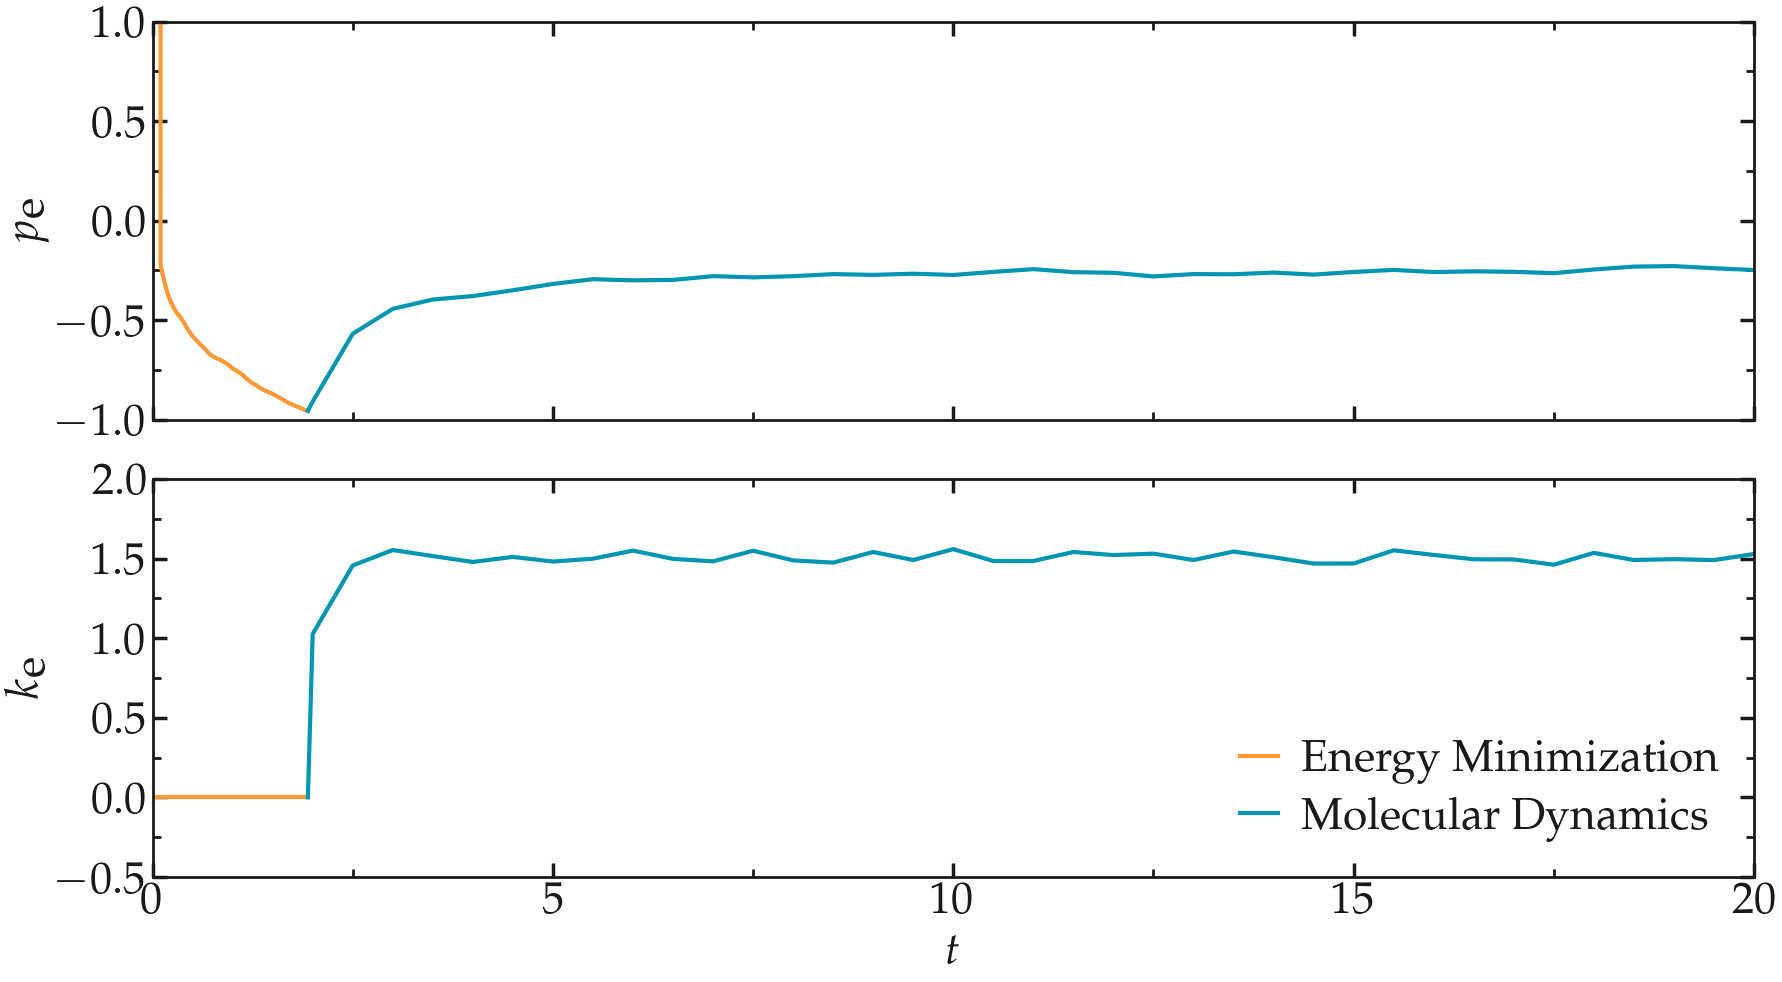
\includegraphics[width=\linewidth]{tutorials/level0/lennard-jones-fluid/energy-light.png}
\end{figure}

\begin{tcolorbox}[colback=mylightblue!5!white,colframe=mylightblue!75!black,title=On the necessity of plotting data efficiently]
When testing/debugging a molecular simulation, it is crucial to be able to control 
on-the-fly the outputs such as the energy to make sure the
system is behaving as expected. If you don't already have 
a favorite plotting tool, you can use xmgrace and simply type from the terminal:
\begin{lcverbatim}
xmgrace energy.dat
\end{lcverbatim}

\noindent This command will automatically plot the second column as a function of the first column.
Here I am using pyplot for esthetic reason. If you want, you can download the Jupyter-notebook
from the \href{https://github.com/lammpstutorials/lammpstutorials.github.io/tree/version2.0/docs/inputs}{the inputs folder} repository (in the \textit{level0/lennard-jones-fluid/} folder).
\end{tcolorbox}

\noindent \section{Trajectory visualisation}

\hspace{-0.45cm}\begin{wrapfigure}{r}{4cm}
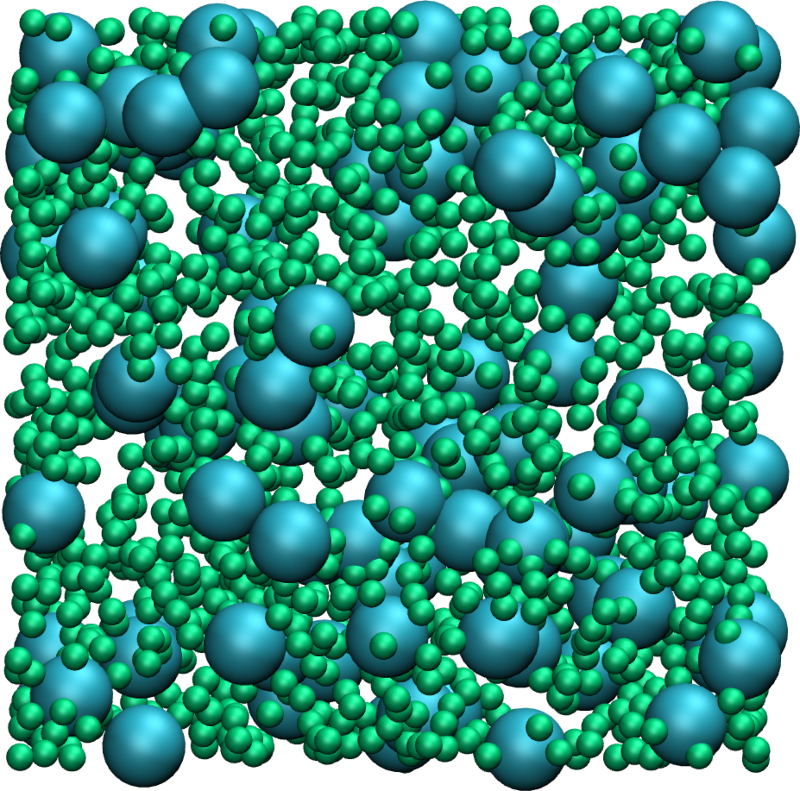
\includegraphics[width=4cm]{tutorials/level0/lennard-jones-fluid/input1.png}
\end{wrapfigure}

\noindent The simulation is running well, but we would like to
visualize the trajectories of the atoms. To do so, we need
to dump the positions of the atoms in a file at a regular
interval. Add the following command in the \textit{visualization}
section of PART B:

\begin{lcverbatim}
dump mydmp all atom 1000 dump.lammpstrj
\end{lcverbatim}

\noindent Run LAMMPS again. A file named \textit{dump.lammpstrj} must appear in
the same folder as your input. This file can be opened using
VMD or Ovito. In Ubuntu, if VMD is installed, you can simply
execute in the terminal:

\begin{lcverbatim}
vmd dump.lammpstrj
\end{lcverbatim}

\noindent Otherwise, you can open VMD and import the \textit{dump.lammpstrj}
file manually using file $\rightarrow$ molecule. You should see a cloud
of lines, but you can improve the representation and make it
look like the figure on the right, or the video at the 
top of this page. 

\section{Improving the script}

\noindent Let us improve the input script and perform slightly more
advanced operations.

\hspace{-0.45cm}\begin{wrapfigure}{r}{4cm}
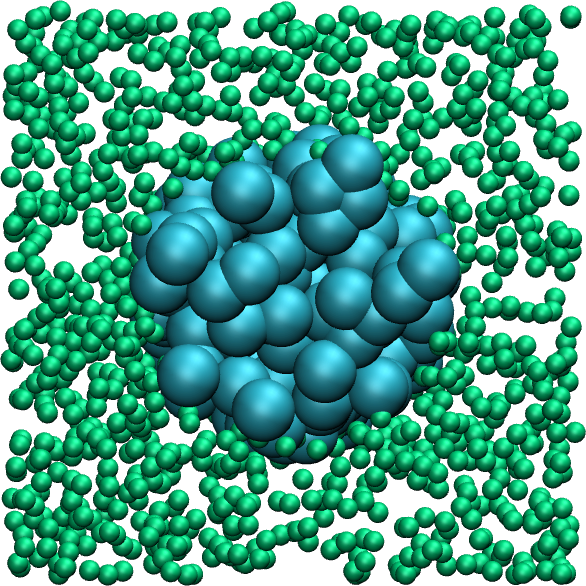
\includegraphics[width=4cm]{tutorials/level0/lennard-jones-fluid/input2.png}
\end{wrapfigure}

\noindent \subsection{Control the initial atom positions}

Let us create the atoms of type 1 and 2 in two separate
regions, respectively, instead of creating them both randomly 
within the entire space as we did previously. Create a new input script, and call
it \textit{input2.lammps}. Similarly to what has been done previously, copy the following lines
into the input script:

\begin{lcverbatim}
# 1) Initialization
units lj
dimension 3
atom_style atomic
pair_style lj/cut 2.5
boundary p p p
\end{lcverbatim}

\noindent Let us create a box from a predefined region,
and create two additional regions and generate
atoms of type 1 and 2 in each region respectively.

\begin{lcverbatim}
# 2) System definition
region simulation_box block -20 20 -20 20 -20 20
create_box 2 simulation_box
region mycylin cylinder z 0 0 10 INF INF side in
region mycylou cylinder z 0 0 10 INF INF side out
create_atoms 1 random 1000 341341 mycylou
create_atoms 2 random 150 127569 mycylin
\end{lcverbatim}

\noindent The \textit{side in} and \textit{side out} keywords
allow us to define regions that are respectively inside the
cylinder, and everything that is not inside the cylinder.
We can write the remaining of the input script as follow:

\begin{lcverbatim}
# 3) Simulation settings
mass 1 1
mass 2 1
pair_coeff 1 1 1.0 1.0
pair_coeff 2 2 0.5 3.0
neigh_modify every 1 delay 5 check yes
# 4) Visualization
thermo 10
dump mydmp all atom 10 dump.min.lammpstrj
# 5) Run
minimize 1.0e-4 1.0e-6 1000 10000
write_data minimized_coordinate.data
\end{lcverbatim}

\noindent The novelty with respect to the previous
input script is the command \textit{write$\_$data}. This command
asks LAMMPS to print the final state of the simulation in
a file named \textit{minimized$\_$coordinate.data}. This file will
be used later to restart the simulation from the final
state of the energy minimisation step.
Run LAMMPS using the \textit{input2.lammps} script. If everything
goes well, a dump file named \textit{dump.min.lammpstrj} will
appear in the folder, allowing you to visualize the atoms
trajectories during minimization. In
addition, a file named \textit{minimized$\_$coordinate.data} will be
created. If you open this file, you will see that it
contains all the information necessary to restart the
simulation, such as the number of atoms and the size of
the box:

\begin{lcverbatim}
1150 atoms
2 atom types
-20 20 xlo xhi
-20 20 ylo yhi
-20 20 zlo zhi
\end{lcverbatim}

\noindent The \textit{minimized$\_$coordinate.data} file also contains the final
positions and velocities of all the atoms:

\begin{lcverbatim}
Atoms # atomic
345 1 -2.8836527978635523e+01 -2.9323791349242530e+01 0.0000000000000000e+00 0 0 0
979 1 -2.9382597284003467e+01 -2.8335352105920894e+01 0.0000000000000000e+00 0 0 0
435 1 -2.5412729704650008e+01 -2.9697644643809667e+01 0.0000000000000000e+00 0 0 0
533 1 -2.5033422381244598e+01 -2.8519424750144708e+01 0.0000000000000000e+00 0 0 0
347 1 -2.4330866813628781e+01 -2.9373591404712414e+01 0.0000000000000000e+00 0 0 0
448 1 -2.3610197298718113e+01 -2.8518785172533800e+01 0.0000000000000000e+00 0 0 0
(...)
\end{lcverbatim}

\noindent The columns of the Atoms section
correspond (from left to right) to the atom indexes (from 1
to the total number of atoms, 1150), the atom types (1 or 2
here), the atoms positions $x$, $y$, $z$ and the
atoms velocities $v_x$, $v_y$, $v_z$.

\subsection{Restarting from a saved configuration}

\noindent We are going to create a new input file and start a
molecular dynamics simulation directly from the previously
saved configuration. In the same folder, create a new file
named input3.lammps and copy the same lines as previously:

\begin{lcverbatim}
# 1) Initialization
units lj
dimension 3
atom_style atomic
pair_style lj/cut 2.5
boundary p p p
\end{lcverbatim}

\noindent Now, instead of creating a new region and adding atoms, we
simply add the following command:

\begin{lcverbatim}
# 2) System definition
read_data minimized_coordinate.data
\end{lcverbatim}

\noindent By visualizing the previously generated dump.min.lammpstrj
file, you may have noticed that some atoms have moved from
one region to the other during minimisation, as seen in
\href{https://www.youtube.com/embed/gfJ_n33-F6A}{this video}.
In order to start the simulation from a clean state, with
only atoms of type 2 within the cylinder and atoms of type
1 outside the cylinder, let us delete the misplaced atoms
by adding the following commands:

\begin{lcverbatim}
region mycylin cylinder z 0 0 10 INF INF side in
region mycylou cylinder z 0 0 10 INF INF side out
group mytype1 type 1
group mytype2 type 2
group incyl region mycylin
group oucyl region mycylou
group type1in intersect mytype1 incyl
group type2ou intersect mytype2 oucyl
delete_atoms group type1in
delete_atoms group type2ou
\end{lcverbatim}

\noindent These commands will respectively recreate
the previously defined regions (regions are not saved by the
\textit{write$\_$data} command), create groups, and finally delete the
atoms of type 1 that are located within the cylinder, as
well as the atoms of type 2 that are located outside the
cylinder. If you run LAMMPS, you can see in the terminal how
many atoms are in each group, and how many atoms have been
deleted:

\begin{lcverbatim}
1000 atoms in group mytype1
150 atoms in group mytype2
149 atoms in group incyl
1001 atoms in group oucyl
0 atoms in group type1in
1 atoms in group type2ou
Deleted 0 atoms, new total = 1150
Deleted 1 atoms, new total = 1149
\end{lcverbatim}

\noindent Similarly to previously, add the following simulation
settings:

\begin{lcverbatim}
# 3) Simulation settings
mass 1 1
mass 2 1
pair_coeff 1 1 1.0 1.0
pair_coeff 2 2 0.5 3.0
neigh_modify every 1 delay 5 check yes
group type1 type 1
group type2 type 2
# 4) Visualization
thermo 1000
dump mydmp all atom 1000 dump.run.lammpstrj
\end{lcverbatim}

\noindent Note that 2 atom groups have been defined, they are useful
here to extract the coordination number between atoms of
type 1 and 2. Let us extract this coordination number, as
well as the number of atoms of each type in each region, by
adding the following commands to the input file:

\begin{lcverbatim}
variable Ntype1in equal count(mytype1,mycylin)
variable Ntype1ou equal count(mytype1,mycylou)
variable Ntype2in equal count(mytype2,mycylin)
variable Ntype2ou equal count(mytype2,mycylou)
fix myat1 all ave/time 10 200 2000 v_Ntype1in v_Ntype1ou file population1vstime.dat
fix myat2 all ave/time 10 200 2000 v_Ntype2in v_Ntype2ou file population2vstime.dat
\end{lcverbatim}

\noindent As seen previously, the fix ave/time
allow to evaluate previously defined variables and print
the values (here every 2000 steps, after averaging each quantities 200 times)
into data file. The 4 variables starting with \textit{Ntype} are used to count
the number of atoms of a specific group in a specific
region. 
Let us also extract the coordination number per atom between atoms 
of type 1 and 2, i.e. the average number of atoms of type 2 in the vicinity 
of the atoms of type 1. This coordination number will be used as an indicator of the 
degree of mixing of our binary mixture. 

\begin{lcverbatim}
compute coor12 type1 coord/atom cutoff 2.0 group type2
compute sumcoor12 all reduce ave c_coor12
fix myat3 all ave/time 10 200 2000 c_sumcoor12 file coordinationnumber12.dat

\end{lcverbatim}

\noindent The \textit{compute ave} is used to average the per atom
coordination number that is calculated by the \textit{coord/atom} compute.
This averaging is necessary as \textit{coord/atom} returns an array where each value corresponds 
to a certain couple of atom i-j. Such array can't be printed by \textit{fix ave/time}. 
Finally, let us complete the script by adding the run section:

\begin{lcverbatim}
# 5) Run
velocity all create 1.0 4928459 mom yes rot yes dist gaussian
fix mynve all nve
fix mylgv all langevin 1.0 1.0 0.1 1530917 zero yes
timestep 0.005
run 300000
write_data mixed.data
\end{lcverbatim}

\noindent There are a few differences with the
previous input script. First, the \textit{velocity create}
command attributes an initial velocity to all the atoms.
The initial velocity is chosen so that the initial
temperature is equal to 1 (unitless). The additional
keywords ensure that no linear momentum and no angular
momentum are given to the system, and that the generated
velocities are distributed as a Gaussian. Another novelty
is the \textit{zero yes} keyword in the Langevin thermostat, that
ensures that the total random force is equal to zero.
After running the simulation, you can observe the number
of atoms in each region from the generated data files, as
well as the evolution of the coordination number due to
mixing:

\begin{figure}
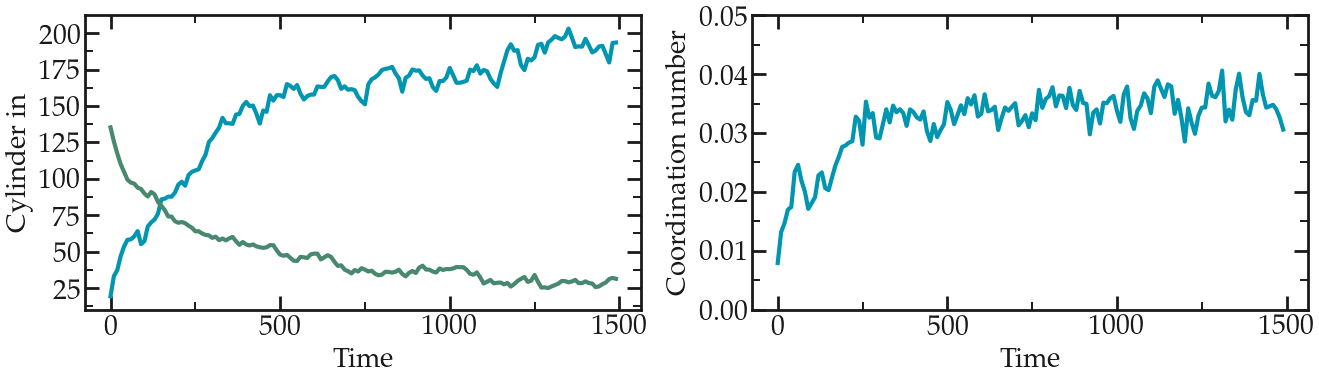
\includegraphics[width=\linewidth]{tutorials/level0/lennard-jones-fluid/population-light.png}
\end{figure}

\section{What now?}

\noindent Now that you have completed this simple molecular dynamics tutorials, what can you do?

\subsection{Play around}

\noindent A good way to progress with LAMMPS and molecular dynamics
simulations is to play around with a script that is already
working and observe the differences and/or errors occurring:
Try adding new commands (you can choose from the documentation),
try removing some of the commands, try changing the parameter values
(see also the first exercise below).
The more you trigger warnings, the easier it will be for you to solve your
own simulation.

\subsection{Try another tutorial}

\noindent There are many common aspects of molecular simulations that were not dealt with in this
tutorial:
\begin{itemize}
\item dealing with charged atoms and bounded molecules, as is necessary to model most existing molecules, solids, or structures, see for instance :ref:`all-atoms-label` and :ref:`sheared-confined-label`,
\item dealing with non-constant volume,
\item dealing with reactivity and bond formation/breaking, see :ref:`reactive-silicon-dioxide-label`.
\end{itemize}

\section{Exercises}

\noindent \subsection{A simulation with no thermostat}

So far, simulations were made using the NVT ensemble [constant number 
of atoms, N, constant volume V, and constant (or at least imposed)
temperature T].
Run a similar simulation in the NVE ensemble, and extract the
total energy of the system over time.

\begin{tcolorbox}[colback=mylightblue!5!white,colframe=mylightblue!75!black,title=Expected output]
Make sure that the total energy is conserved over time, as see here. Note also 
that the kinetic energy constantly exchanges with the potential energy.
\end{tcolorbox}

\noindent \subsection{Do without the *minimize* command}

Run a successful simulation without using the \textit{minimize} command.
The absence of energy minimization needs to be compensated
in order to avoid triggering the \textit{ERROR: Lost atoms} message.

\begin{tcolorbox}[colback=mylightblue!5!white,colframe=mylightblue!75!black,title=Hints]
The value of the timestep and/or the damping factor of the fix langevin
can be tuned to prevent the system from exploding.
Perform as many consecutive runs with varying timestep and damping
factors that you feel are necessary.
Have a look at fix nve/limit. This command was
made to prevent an unequilibrated system from exploding
by preventing atoms to travel too far every timestep.
\end{tcolorbox}

\noindent \subsection{Non-equilibrium simulation}

So far, atoms were freely diffusing without contraint or external force.
Add an external force to induce a net flow of atoms in one
direction. The magnitude of the force must be chosen so
that the system is not \textit{too far} from equilibrium.

\begin{tcolorbox}[colback=mylightblue!5!white,colframe=mylightblue!75!black,title=Hints]
LAMMPS offers several option to add external force to a system, one 
being the fix addforce.
Note: If the system is too far from equilibrium, it enters the non-linear response 
regimes and its properties and parameters will differ from its equilibrium values.
In general, this is something that you must avoid (unless you are studying
non-linear effects). 
\end{tcolorbox}

\noindent \subsection{Dumbbell molecules}

Add a bond between couple of identical atoms to create
dumbbell molecules, just like in the image:

\begin{figure}
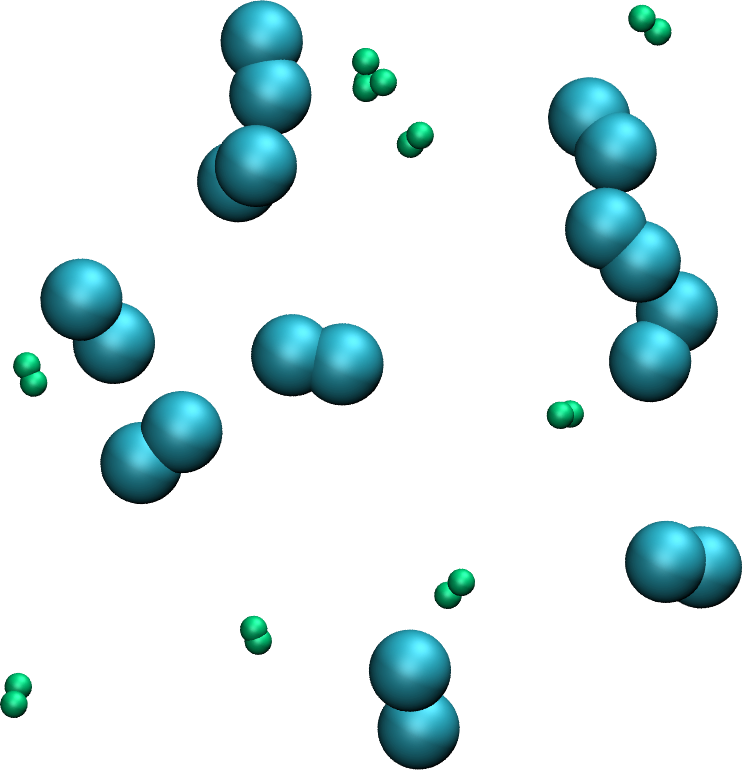
\includegraphics[width=\linewidth]{tutorials/level0/lennard-jones-fluid/dumbell-light.png}
\end{figure}

\begin{tcolorbox}[colback=mylightblue!5!white,colframe=mylightblue!75!black,title=Hints]
Use molecule template to easily insert as many atoms connected
by bonds (i.e. molecules) as you want. A molecule 
template typically begins as follow:
\begin{lcverbatim}
# Dumbell molecule
2 atoms
1 bonds
Coords
1 0.5 0 0
2 -0.5 0 0
(...)
\end{lcverbatim}

\noindent \end{tcolorbox}

